% Created 2024-02-16 ven. 16:17
% Intended LaTeX compiler: pdflatex
\documentclass[11pt]{article}
\usepackage[utf8]{inputenc}
\usepackage[T1]{fontenc}
\usepackage{graphicx}
\usepackage{longtable}
\usepackage{wrapfig}
\usepackage{rotating}
\usepackage[normalem]{ulem}
\usepackage{amsmath}
\usepackage{amssymb}
\usepackage{capt-of}
\usepackage{hyperref}
\usepackage[T1]{fontenc}
\usepackage{lmodern}
\usepackage[font=small,labelfont=bf, justification=justified, format=plain]{caption}
\author{J.-M. Chauvet}
\date{\today}
\title{Memory GAPS: Are LLMs Tulving-Complete?}
\hypersetup{
 pdfauthor={J.-M. Chauvet},
 pdftitle={Memory GAPS: Are LLMs Tulving-Complete?},
 pdfkeywords={},
 pdfsubject={},
 pdfcreator={Emacs 28.2 (Org mode 9.6.3)}, 
 pdflang={English}}
\begin{document}

\maketitle

\section*{Abstract}
\label{sec:org16358fb}
\section*{Introduction}
\label{sec:org5832e2c}
In his groundbreaking studies of memory, Endel Tulving (1927-2023) noted that "one of the most compelling and salient characteristics of remembering of past events is the individual's subjective awareness of remembering" (Endel Tulving, 1983). In order to include the rememberer's recollective experience into the critical constructs in the conceptualization of remembering, Tulving suggested an "overall pretheoretical framework", called the \emph{General Abstract Processing System} or GAPS. This paper investigates whether the GAPS also provides insights when the subject is no longer human but a Large Language Model (LLM).

Tulving championed the distinction of \emph{episodic} from \emph{semantic} memory, successfully arguing that being functionnally different, they represent separate but related systems. Both are placed on the same side of the cognitive division between \emph{declarative memory} (as episodic and semantic information can be expressed through language--e.g. repairing a bicycle) on the one hand, and \emph{skills} (which can be observed only in behavior--e.g. riding a bicycle) on the other.

\subsection*{The GAPS and the Transformer}
\label{sec:org9d30808}
In Tulving's framework, a single act of remembering forms the unit of human episodic memory. Remembering is a process that begins with the witnessing or experiencing of an episode and ends with its recollective experience or with the conversion of the remembered information into some other form, or both. The GAPS specifies so called \emph{elements} of remembering and their interrelations in order to decompose this process.

The GAPS distinguishes two kinds of elements: observable events and hypothetical constructs (processes and states); and it divides elements into two categories: elements of encoding and elements of retrieval.

\begin{figure}[htbp]
\centering
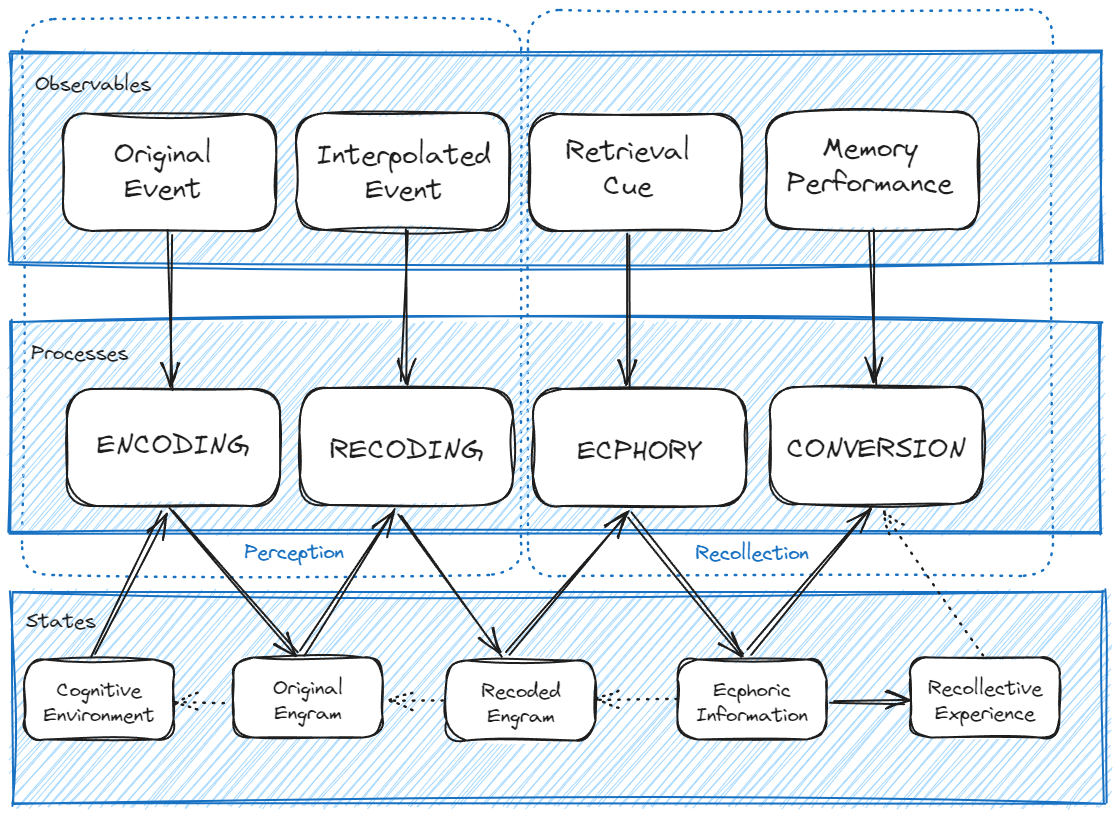
\includegraphics[width=.9\linewidth]{ElementsOfRemembering-rev.png}
\caption{\label{fig:org2061eec}\textbf{The GAPS: Elements of Episodic Memory and their Relations.} The element of encoding is a process that converts the information about an experienced event or episode (in a particular setting, at a particular time) into an \emph{engram} or memory trace. The central element of the retrieval processes \emph{ecphoric} information, a synergistic product of the engram and the retrieval cue, which calls on both episodic and semantic information. Source for figure: (Endel Tulving, 1983 Ch. 7, Fig. 7-1, p. 135).}
\end{figure}

Of particular interest to this study of applicability of the GAPS framework to LLM are the possible transpositions of engram and ecphoric information into the domain of generative AI. In his seminal book, Tulving offers a very broad definition of engrams: "the product of encoding", "conditions for recollection of the experienced event", or "differences between the state of the memory system before and after encoding". The latter is closely related the original definitions of these terms introduced by Richard Semon (1859--1918): "to represent the enduring changes brought about by the energetic effect of stimuli in the organism" (Daniel L. Schacter and James Eric Eich and Endel Tulving, 1978, Semon, Richard Wolfgang, 1920). Note that if, in both clarifications, the nature of the changes are unknown, the term became nonetheless broadly known in psychology research through the later work of Karl Lashley (1890--1958) concluding, amongst other experimental results on neural mechanisms involved in learning and memory, that "there is no demonstrable localization of memory trace" (Lashley, Karl S, 1950).

Similarly inspired by Semon, Tulving suggested the terms \emph{ecphory} and \emph{ecphoric information} to designate respectively the process that brings (i) the relevant information in the retrieval environment into interaction with (ii) the original or recoded engram, and the output of this process. Such ecphoric information determines the particulars of recollective experience in the next phase of remembering: \emph{conversion}. In the GAPS model, ecphoric information is basically a task-free component of the retrieval process, it is simply used by being converted into another form in the memory performance.

The categories of encoding and retrieval in the GAPS are not without analogies with the \emph{Transformer} architecture of neural networks at the core of LLMs, which precisely articulates encoders and decoders to process vector embeddings representing words and sentences.

\begin{figure}[htbp]
\centering
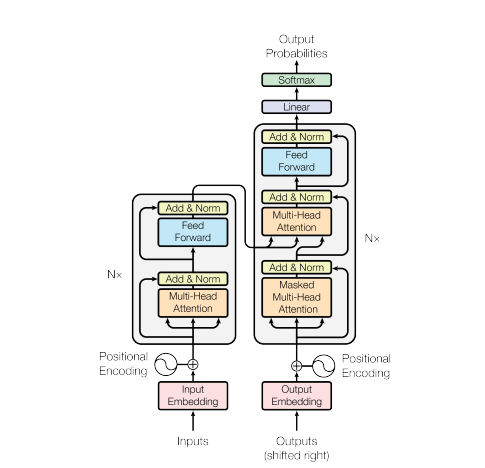
\includegraphics[width=.9\linewidth]{Transformer.png}
\caption{\label{fig:orgbce2a07}\textbf{The Transformer Architecture.} Based on the 2017 paper (Vaswani, Ashish, Shazeer, Noam, Parmar, Niki , Uszkoreit, Jakob, Jones, Llion, Gomez, Aidan N., Kaiser, Łukasz, Polosukhin, Illia, 2017) attention mechanism, the Transformer architecture requires less training time than previous recurrent neural architectures. Input text is split into tokens (sometimes called \emph{n-gram}, dangerously reminiscent of Semon's engrams--see text), then converted into vectors. Through different layers, each token is contextualized with other tokens via parallel attention heads, calculating weights for each according to its importance. The Transformer Architecture elaborates on \emph{softmax-based} attention mechanism (Dzmitry Bahdanau, Kyunghyun Cho, Yoshua Bengio, 2014) and \emph{Fast Weight Controllers} (Imanol Schlag, Kazuki Irie, Jürgen Schmidhuber, 2021). Source for figure: (Vaswani, Ashish, Shazeer, Noam, Parmar, Niki , Uszkoreit, Jakob, Jones, Llion, Gomez, Aidan N., Kaiser, Łukasz, Polosukhin, Illia, 2017).}
\end{figure}

At this stage, from cursorily reviewing the architecture of both GAPS and Transformer--and keeping in mind that Tulving's psychological framework is only "pre-theoretical" and "highly schematic", while Transformers are actual computer implementations--the practical analogy would unfold as follows:

\begin{table}[htbp]
\caption{\label{tab:org3646b5e}\textbf{Hypothetical analogy between GAPS and Transformer.} Semantic memory, in Tulving's acception, would be represented by the probability distribution learned by the LLM during the pretraining phase. In Transformers it determines the particulars of the output based on the input (prompt).}
\centering
\begin{tabular}{lll}
 & GAPS & Transformer\\[0pt]
\hline
Processes & encoding & encoder\\[0pt]
 & recoding & encoder\\[0pt]
 & ecphory & encoder\\[0pt]
 & conversion & decoder\\[0pt]
\hline
States & engram & vector embedding\\[0pt]
 & ecphoric information & output probabilities\\[0pt]
 & memory performance & output\\[0pt]
\end{tabular}
\end{table}

\subsection*{Tulving's "direct comparison": recognition versus recall}
\label{sec:orgdc7f125}
In order to further investigate the analogy and its grounds, we adopt Tulving's design of "direct comparison" experiments to assess recognition versus recall tasks in LLMs. Recogniton and recall are both processes of retrieval and both results in the rememberer's awareness of a past event. The simple episodes in the experiment are to be presentations of a list of english words to be remembered. In this simplified situation of comparing recognition and recall tasks, we consider only two independent dimensions: one has to do with the type of retrieval information, or \emph{cue}, available to the rememberer; the second refers to the conversion process in the GAPS framework. The retrieval information includes copies of the studied words and non-copy cue words. As for the conversion process: in the recognition task, the rememberer has to express whether or not the cue word was in the study list (\emph{familiarity}); in the recall task, the rememberer has to identify a word in the study list, if any, associated with the cue word (\emph{identification}), thereby expressing some other aspect of the original memorizing experience. Note that in the GAPS framework, the first dimension involves processes anterior to the construction of ecphoric information, while the second relates to post-ecphoric processes. The experimental results are therefore captured by the 2 x 2 matrix in Table \ref{tab:org3069956}

\begin{table}[htbp]
\caption{\label{tab:org3069956}Differences between recognition and recall tasks. Source for table: (Endel Tulving, 1983 Ch. 14).}
\centering
\begin{tabular}{lll}
Retrieval information & Conversion & \\[0pt]
 & Familiarity & Identification\\[0pt]
\hline
Copy Cue Word & \emph{Recognition} & ?\\[0pt]
Non-Copy Cue Word & ? & \emph{Recall}\\[0pt]
\end{tabular}
\end{table}

Conventional recognition and recall tests sit in two of the four cells in the matrix. When the rememberer, however, declares a cue other than a copy cue word to be familiar it is a \emph{false positive} response from the conventional perspective although psychologist might disagree on how to think about such responses (Moshe Anisfeld and Margaret Knapp, 1968). The other empty cell represents a situation where the rememberer's somewhat strange task is to repeat the cue word to confirm it associates with the copy in the study list. \emph{False negatives} are of interest here and Tulving's interpretation was that these entailed a form of continuity between recognition and recall retrieval processes.

The direct comparison test design represents all four cells of the matrix. In a typical session the LLM is prompted to memorize a list of 48 common english words. In a group of experiments, the LLM is prompted with a cue word and asked whether the cue is included or not in the studied list; in another group, the LLM is prompted with a cue word and asked to retrieve any strongly associated word in the studied list (or none if no such word is evoked by the cue).

In order to introduce the distinction between immediate and delayed retrieval of the original experimental design, the experiment is run twice for each group: in the first run, memorization and retrieval are both in each individual prompt (immediate); in the second, memorization is the first prompt of a conversation (chat) with the LLM, followed by retrieval prompts which continue the conversation (delayed).

\section*{Results}
\label{sec:org72ac89b}
As a reference benchmark, the results of Tulving's original experiments are presented in Table \ref{tab:org3e795ed} from (Endel Tulving, 1983 Ch. 14, Table 14.2):

\begin{table}[htbp]
\caption{\label{tab:org3e795ed}\textbf{Summary of memory performance in the 'direct comparison' experiment.} Each proportion shown is based on 576 observations. The data for the familiarity (recognition) task show proportion of cases in which the human subjects regarder the cue word as included in the list. Hence the data for copy cues represent 'correct' responses, whereas the data from the other three types of cues represent 'false positives'. The data for the indetification (recall) task indicate proportions of responses to the cue being any target word in the list.}
\centering
\begin{tabular}{l|rr|rr}
Retrieval information & Conversion &  &  & \\[0pt]
 & Familiarity &  & Identification & \\[0pt]
 & Immediate & Delayed & Immediate & Delayed\\[0pt]
\hline
Copy Cue Word & 0.78 & 0.71 & 0.69 & 0.60\\[0pt]
Non-Copy Associated & 0.15 & 0.20 & 0.54 & 0.37\\[0pt]
Non-copy Rhyme & 0.09 & 0.15 & 0.20 & 0.31\\[0pt]
Non-copy Unrelated & 0.08 & 0.18 & 0.04 & 0.02\\[0pt]
\end{tabular}
\end{table}




\section*{Discussion}
\label{sec:org0975b3d}

Compare to Estes' short/long-term memomy in human and computer discussion (Estes, W K, 1980).
\begin{quote}
By contrast, the results of research in my laboratory (Estes 1972; Lee and Estes 1977) suggest that human short-term memory is quite differ ently organized, being oriented toward events and their* attributes rather than toward the retention of items as units. In the human memory, forgetting is characteristically a pro gressive loss of precision of informa tion about an event rather than a matter of total recall or total loss of a stored item.
\end{quote}

\section*{Methods}
\label{sec:org07d19e2}
We transpose the 'direct comparison' experiment, between recognitin and recall, described in (Endel Tulving, 1983 Chapter 14) to LLM subjects.
\section*{References}
\label{sec:orgf05cc35}

\noindent
Daniel L. Schacter and James Eric Eich and Endel Tulving (1978). \emph{Richard Semon's theory of memory}, Journal of Verbal Learning and Verbal Behavior.

\noindent
Dzmitry Bahdanau, Kyunghyun Cho, Yoshua Bengio (2014). \emph{Neural Machine Translation by Jointly Learning to Align and Translate}.

\noindent
Endel Tulving (1983). \emph{Elements of Episodic Memory}, Oxford University Press.

\noindent
Estes, W K (1980). \emph{Is human memory obsolete?}, Am Sci.

\noindent
Imanol Schlag, Kazuki Irie, Jürgen Schmidhuber (2021). \emph{Linear Transformers Are Secretly Fast Weight Programmers}.

\noindent
Lashley, Karl S (1950). \emph{In search of the engram.}, Academic Press.

\noindent
Moshe Anisfeld and Margaret Knapp (1968). \emph{Association, Synonymity, and Directionality in False Recognition}, Journal of Experimental Psychology.

\noindent
Semon, Richard Wolfgang (1920). \emph{Die Mneme als erhaltendes Prinzip im Wechsel des organischen Geschehens}, Engelmann.

\noindent
Vaswani, Ashish, Shazeer, Noam, Parmar, Niki , Uszkoreit, Jakob, Jones, Llion, Gomez, Aidan N., Kaiser, Łukasz, Polosukhin, Illia (2017). \emph{Attention is all you need}, Curran Associates Inc..

\section*{Acknowledgements}
\label{sec:org247a649}
\section*{Author information}
\label{sec:orgee940d7}
\section*{Ethics declarations}
\label{sec:org0a000ee}
\section*{Additional information}
\label{sec:org9a3dcb9}
\section*{Electronic supplementary material}
\label{sec:orgbd84ddc}
\section*{Rights and permissions}
\label{sec:org7695766}
\section*{About this article}
\label{sec:org79353ae}
\section*{Further reading}
\label{sec:org1ec517f}
\section*{Comments}
\label{sec:org3b5b72a}
\end{document}